
% !TEX useTabs

\documentclass[12pt,oneside]{book}
\usepackage{amsmath}
\usepackage{amssymb}
\usepackage{bm}
\usepackage{epsfig}
\usepackage{graphicx}
\usepackage{color}
\usepackage[colorlinks=true]{hyperref}

\usepackage[russian]{babel}

\addto\captionsrussian{\renewcommand{\chaptername}{Лекция}}
\def\dfrac{\displaystyle\frac}
\newcommand{\rot}{\mathop{\rm rot}\nolimits}
\newcommand{\Sp}{\mathop{\rm Sp}\nolimits}
\newcommand{\St}{\mathop{\rm St}\nolimits}
\newcommand{\erf}{\mathop{\rm erf}\nolimits}
\newcommand{\arch}{\mathop{\rm Arch}\nolimits}
\newcommand{\floor}{\mathop{\rm floor}\nolimits}
\renewcommand{\Re}{\mathop{\rm Re}}
\renewcommand{\Im}{\mathop{\rm Im}}

\renewcommand{\theequation}{\arabic{chapter}.\arabic{equation}}
\renewcommand{\chaptermark}[1]{\markright{\thechapter.\ #1}}
\renewcommand{\chaptermark}[1]{\markright{#1}}


\usepackage[]{nomencl}
\setlength{\nomitemsep}{-0.1cm}
\addto\captionsrussian{\renewcommand{\nomname}{Список основных обозначений}}
\makenomenclature

\newcommand{\add}[1]{\textcolor{magenta}{#1}}


\usepackage{dsfont}%мат. символы
\usepackage{amsmath} %common math symbols

\begin{document}
\title{Работа}
\author{Сингалевич Дмитрий}
\date{01.01.2022}
\maketitle

\section{Прецессия спина}
	
	{Спин электрона в магнитном поле прецессирует согласно уравнению прецессии:\\
	\begin{equation}
		\label{Bloh}
		\frac{\bm {dS}}{dt} = [ \bm \Omega \times \bm{S}] ,
	\end{equation}
	где $ \bm{S}$ - спин электрона, $\bm{S}=\hbar\bm{\sigma}/2$.	
	А угловая скорость прецессии $\bm \Omega$ связана с магнитным полем гиромагнитным коэффициентом:
	\begin{equation}
		\label{Effective} 
		{\bm{\Omega _k}} = \gamma{{\bm{B}}_k} = g\frac{{\left| e \right|{{\bf{B}}_{\bf{k}}}}}{{2{m_0}c}}  ,
	\end{equation}
	где g - аномальный g-фактор электрона, ${m_0}$ - масса электрона.
	\\
	Это уравнение можно спроецировать по осям:
	$$\begin{cases}
		\Dot{S_x} = \Omega_y{S_z} - \Omega_z{S_y} \\
		\Dot{S_y} = \Omega_z{S_x} - \Omega_x{S_z} \\
		\Dot{S_z} = \Omega_x{S_y} - \Omega_y{S_x}
	\end{cases}$$
	При решении смешанным численным методом эта система преобразуется:
	$$\begin{cases}
		\frac{S_x(t+dt) - S_x(t)}{dt} = \Omega_y\frac{S_z(t+dt) + S_z(t)}{2} - \Omega_z\frac{S_y(t+dt) + S_y(t)}{2} \\
		\frac{S_y(t+dt) - S_y(t)}{dt} = \Omega_z\frac{S_x(t+dt) + S_x(t)}{2} - \Omega_x\frac{S_z(t+dt) + S_z(t)}{2} \\
		\frac{S_z(t+dt) - S_z(t)}{dt} = \Omega_x\frac{S_y(t+dt) + S_y(t)}{2} - \Omega_y\frac{S_x(t+dt) + S_x(t)}{2}
	\end{cases}$$
	Перегруппировка слагаемых: 
	$$\begin{cases}
		{S_x(t+dt)}+{{\frac{1}{2}\Omega_z{dt}}\cdot{S_y(t+dt)}}-{{\frac{1}{2}\Omega_y{dt}}\cdot{S_z(t+dt)}} = {S_x(t)} - {\frac{1}{2}\Omega_z{dt}}\cdot{S_y(t)} + {\frac{1}{2}\Omega_y{dt}}\cdot{S_z(t)} \\
		{{ -\frac{1}{2}\Omega_z{dt}}\cdot{S_x(t+dt)}}+{S_y(t+dt)}+{{\frac{1}{2}\Omega_x{dt}}\cdot{S_z(t+dt)}} = {\frac{1}{2}\Omega_z{dt}}\cdot{S_x(t)} + {S_y(t)} - {\frac{1}{2}\Omega_x{dt}}\cdot{S_z(t)} \\
		{{\frac{1}{2}\Omega_y{dt}}\cdot{S_x(t+dt)}}+{{\frac{1}{2}\Omega_x{dt}}\cdot{S_y(t+dt)}}+{S_z(t+dt)} = -{\frac{1}{2}\Omega_y{dt}}\cdot{S_x(t)} + {\frac{1}{2}\Omega_x{dt}}\cdot{S_y(t)} + {S_z(t)}
	\end{cases}$$
	Для удобства можно переписать эту систему в матричном виде:
	\begin{eqnarray*}
		\begin{pmatrix}
			 1& \frac{1}{2}\Omega_z{dt}& -\frac{1}{2}\Omega_y{dt}\\
			  -\frac{1}{2}\Omega_z{dt}& 1& \frac{1}{2}\Omega_x{dt}\\
			  \frac{1}{2}\Omega_y{dt}& -\frac{1}{2}\Omega_x{dt}& 1
		\end{pmatrix}
		\cdot
		\begin{pmatrix}
			 S_x(t + dt)\\
			 S_y(t + dt)\\
			 S_z(t + dt)
		\end{pmatrix}
		=  \\ =
		\begin{pmatrix}
			 {S_x(t)} - {\frac{1}{2}\Omega_z{dt}}\cdot{S_y(t)} + {\frac{1}{2}\Omega_y{dt}}\cdot{S_z(t)}\\
			 {\frac{1}{2}\Omega_z{dt}}\cdot{S_x(t)} + {S_y(t)} - {\frac{1}{2}\Omega_x{dt}}\cdot{S_z(t)}\\
			 -{\frac{1}{2}\Omega_y{dt}}\cdot{S_x(t)} + {\frac{1}{2}\Omega_x{dt}}\cdot{S_y(t)} + {S_z(t)}
		\end{pmatrix}
	\end{eqnarray*}

\section{Спин-орбитальное взаимодействие}
	%\hspace{10mm}
	{При движении электрона во внешнем элетрическом поле проявляется эффект спин-орбитального взаимодействия:
	спин электрона прецессирует вследствие появления магнитного поля в системе отсчёта электрона.\\
	%пояснить про электромагнитные поля в разных системах отсчета
	\\
	Для свободного электрона в постоянном электрическом поле можно вычислить получившееся магнитное поле по формуле:
	% B =1/c * [E x V]
	\[{{\bm{B}}_k} = \frac{1}{c}[\bm{E} \times \bm{v}]\] .
	\\
	Но при движении электрона в полупроводнике (что означает, что он не свободен) проявляется эффект Рашбы, усиливающий спин-орбитальное взаимодействие. В таком случае принято говорить о спин-орбитальном взаимодействии Рашбы, работающим по закону:
	\begin{equation}
		\label{OmegaR}
		{\Omega_k}\cdot{S} = {\alpha_R(E)}\cdot{k} ,
	\end{equation}
	где ${\alpha_R(E)}$ - коэффициент спин-орбитального взаимодействия, зависящий от электрического поля;
	${k}$ - волновой вектор электрона, вычисляемый из формулы:
	\begin{equation}
		\label{k}
		\bm{v} = \frac{{\hbar \bm{k}}}{m^*} ,
	\end{equation}
	где ${m^*}$ - эффективная масса электрона.
	

\section{Спин в транзисторе}
	Частный случай полета электрона в полупроводнике под действием электрического поля - это полет электрона в транзисторе.
	 Для этого случая будем считать, что  ${\alpha_R}$ прямо пропорционально электрическому полю E с коэффициентом ${r_R}$:
	${\alpha_R} = {r_R}\cdot{E}$ .
	\newline
	Рассмотрим беспрепятственный полет электрона. Тогда ${k = const}$ из чего по формуле \ref{OmegaR} следует, что скорость прецессии постоянна.
	При этом прецессия происходит в одной плоскости и это можно изобразить на схеме (рис. \ref{fig:f1}).
	\begin{figure}[h]
		\centering
		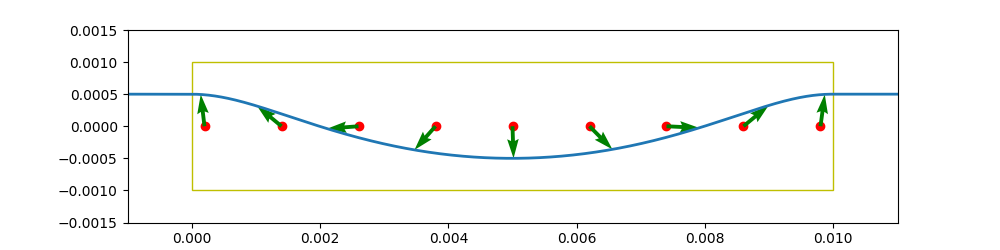
\includegraphics[width = 16cm, height = 4cm]{img/Transistor.png}
		\caption{Прецессия спина в транзисторе. Желтая рамка - границы транзистора.}
		\label{fig:f1}
	\end{figure}
	\newline
	Можно задать такие значения электрического поля E и длины транзистора L, что прецессия произойдет на нужный угол $\beta$. 
	Связь этих величин задается уравнениями \ref{OmegaR} и \ref{k}, а также уравнениями движения электрона и  угловой скорости спина:
	$$\begin{cases}
		{\Omega_k} = \frac{{{r_R}\cdot{E}}\cdot{k_F}}{S} \\
		{v} = \frac{{\hbar}k}{m^*} \\
		{\tau} = \frac{L}{v} \\
		{\beta} = {\Omega_{k}}\cdot{\tau}
	\end{cases}$$
	Из этой системы уравнений можно получить, что:
	\begin{equation}
		\label{beta}
		{\beta} = {\frac{{{r_R}\cdot{E}}\cdot{k_F}}{S}}\cdot{\frac{Lm^*}{{\hbar}k}} = \frac{2{r_R}{m}{E}{L}}{{\hbar}^2}
	\end{equation}
	\newline
	Для прецессии спина на ${\pi}$ произведение ${E}\cdot{L}$ должно равняться: 
	\begin{equation}
		\label{pi}
		{E}\cdot{L} = \frac{{\pi}{\hbar}^2}{2{r_R}{m^*}}
	\end{equation}
	Оценим значения величин в уравнении для квантовой ямы в GaAs: \\
	$r_R\approx{5}\cdot{10}^{-16} \,e\cdot\text{см}^2\approx{2.4}\cdot{10}^{-25}\text{ СГС}\cdot\text{см}^2$ \\
	$m^* \approx {0.1}\cdot{m_0}\approx{9.1}\cdot{10}^{-29}\text{ г}$ \\
	${\hbar}\approx{1.1}\cdot{10}^{-27}\text{ эрг}\cdot\text{с}$ \\
	Тогда: ${E}\cdot{L}\approx{9}\cdot{10}^{-2}\text{ СГС}/\text{см}$ \\
	При длине транзистора ${L = 0.01}$ см : \\
	$E\approx{9}\text{ СГС}/\text{см}^2\approx{2.7}\cdot{10}^{5}\text{ В}/\text{м}$
	

\section{Релаксация спина}
	Спиновой релаксацией называется прецессия спина на достаточно большой угол. Будем брать этот угол равным 1 радиану.
	\newline
	В модели беспрепятственного полета электрона релаксация происходит за время ${1 rad/\Omega}$ . Однако в реальном полупроводнике, вследствие теплового движения ячеек кристалической решетки, электрон постоянно сталкивается с ними и меняет направление своей скорости (а значит и плоскость вращения). Вследствие этого время релаксации становится больше, чем в модели без столкновений (но если столкновения происходят настолько редко, что за время между изменениями вектора скорости спин успеет спрецессиовать на 1 радиан, то время релаксации не изменится). 
	\newline
	\newline
	Для визуализации прецессии спина используется сфера Блоха - трехмерная диаграмма в виде линии, характеризующей перемещения вершины вектора спина, считая что основание вектора - в центре сферы (рис. \ref{fig:f2}).
		\begin{figure}[h!]
		\centering
		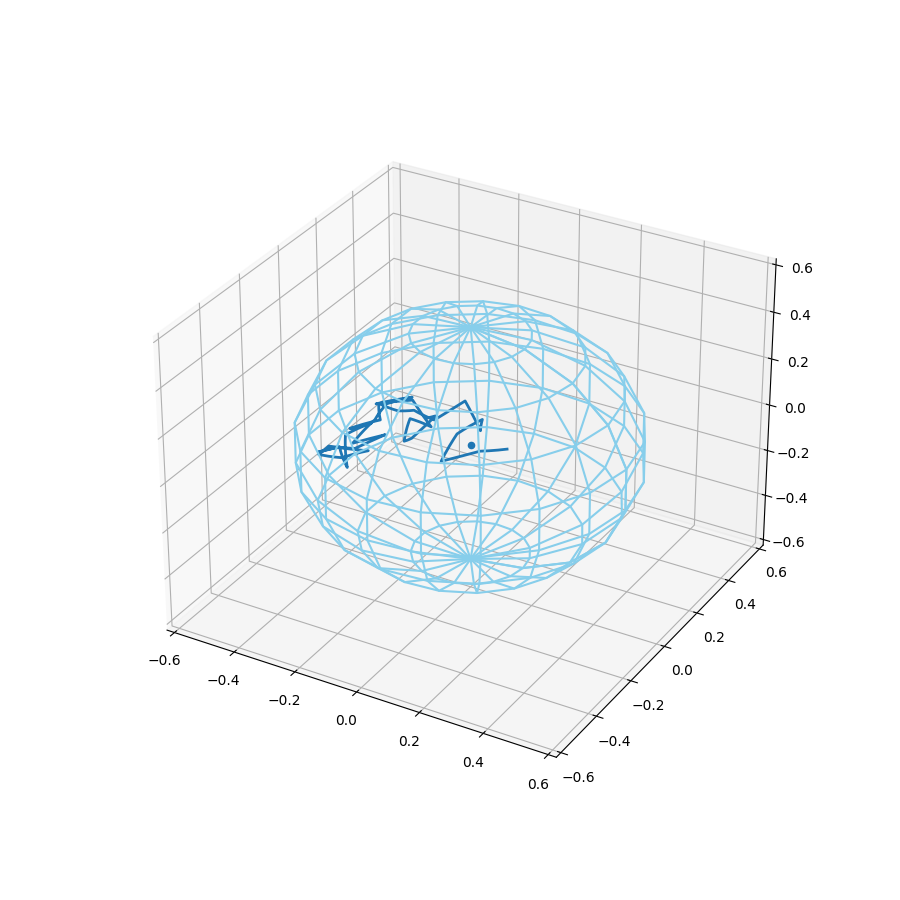
\includegraphics[width = 16cm, height = 16cm]{img/Bloch_Sphere_1.png}
		\caption{Сфера Блоха}
		\label{fig:f2}
	\end{figure} 
	\\
	\\
 	В определенном приближении можно считать, что столкновения происходят через равные промежутки времени, а скорость после каждого столкновения меняет только свое направление на случайное. Заметим, что для любого распределения плотности вероятности по времени между столкновениями можно выбрать такое время $\tau$, что среднее время релаксации в модели равного времени между столкновениями будет таким же, как и в реальности. Также будет рассматриваться исключительно тот случай, когда при входе в полупроводник спин перпендекулярен случайному магнитному полю (то есть первый угловой "шаг" по сфере будет равен ${\Omega}{\tau}$).
	\newline
	\newline
	С помощью программы снимем зависимость времени релаксации $\tau_s$ от времени между столкновениями $\tau$ и построим её график, используя по обеим осям размерность $\frac{1}{\Omega}$ (рис. \ref{fig:f3}).
	\begin{figure}[h!]
		\centering
		\includegraphics[width = 16cm, height = 8.65cm]{img/relaxation_plot.png}
		\caption{Зависимость времени релаксации от времени между столкновениями}
		\label{fig:f3}
	\end{figure} 
	Из графика видно, что при времени между столкновнениями большем, чем $\frac{1}{\Omega}$, время релаксации становится константой. Это объясняется тем, что когда величина ${\Omega}{\tau}$ превышает 1, за время до первого столкновения спин успевает спрецессировать на угол более 1 радиан, а значит релаксация происходит за одно и то же время. При этом это время равно  ${1 rad/\Omega}$, то есть 1 в данных осях.
	\newline
	Построим этот график в двойном логарифмическом масштабе (\ref{fig:f4}). Заметим, что при небольших значениях  ${\Omega}{\tau}$ этот график представляет из себя прямую, а значит что зависимость  $\tau_s(\tau)$ - степенная. Коэффициент наклона этой прямой равен 0.91, откуда  $\tau_s ~ \tau^0.91$. Но при приближении ${\Omega}{\tau}$ к 1 угол наклона уменьшается и становится равен $\approx 0.7$ .
	\begin{figure}[h!]
		\centering
		\includegraphics[width = 16cm, height = 8.55cm]{img/relaxation_log_log_plot.png}
		\caption{Зависимость времени релаксации от времени между столкновениями в двойном логарифмическом масштабе}
		\label{fig:f4}
	\end{figure}
%	Заметим, что прецессия спина при постоянном времени между столкновениями представляет из себя случайное блуждание по сфере (для удобства - радиуса 1). 
%Тогда длина дуги между начальной позицией электрона и его позицией спустя n шагов будет равна радиус вектору такого же блуждания, но по плоскости (при этом шаг на плоскости равен угловому шагу по сфере).
 %Тогда время релаксации $\tau_s$ обратно пропорционально времени между столкновениями $\tau$. Это можно записать как: ${\tau_s}\cdot{\tau} = const$. Заметим, что формула верна только для при малых значениях ${\Omega}{\tau}$ (в этом случае шаг много меньше суммарного перемещения).
%	\newline
%	Построим график ${\tau_s}\cdot{\tau}$ (в осях $\frac{1}{\Omega^2}$) от $\tau$ (в осях $\frac{1}{\Omega}$). При малых значениях $\tau$ величина ${\tau_s}\cdot{\tau}$ примерно равна ${1}\cdot{\frac{1}{\Omega^2}}$, откуда ${{\Omega^2}{\tau_s}{\tau} = 1}$. При увеличении $\tau$ величина ${\tau_s}\cdot{\tau}$ монотонно растет, и при достижении ${\Omega}{\tau} = 1$ резко падает до $\frac{1}{\Omega^2}$. Для больших значений времени между столкновениями график не имеет смысла, так как время релаксации становится константой.


\section{Релаксация спина во внешнем магнитном поле}
	Рассмотрим воздействие внешнего магнитного поля на релаксацию спина. Тогда суммарное значение $\bm{\Omega} = \bm{\omega} + \bm{{\Omega}_{outside}}$ (где ${\omega}$ - случайное магнитное поле от спин-орбитального взаимодействия). При достаточно большом внешнем поле  $\bm{\Omega} \approx \bm{{\Omega}_{outside}}$, и тогда прецессия происходит вокруг оси внешнего поля.
	Рассмотрим случай, когда ${\Omega}_{outside}$ сонаправлена со спином в момент входа в полупроводник. Тогда при увеличении внешнего поля увеличится и время релаксации (т.к. спин вращается вокруг текущего $\bm{\Omega}$, а большое ${\Omega}_{outside}$  делает $\bm{\Omega}$ сонаправленным с начальным положением спина).
	\newline
	В качестве иллюстрации этого процесса можно использовать сферу Блоха при разных внешних полях (\ref{fig:f5}) - чем больше внешнее поле, тем больше время релаксации (тем больше количество витков).
	\begin{figure}[h!]
		\centering
		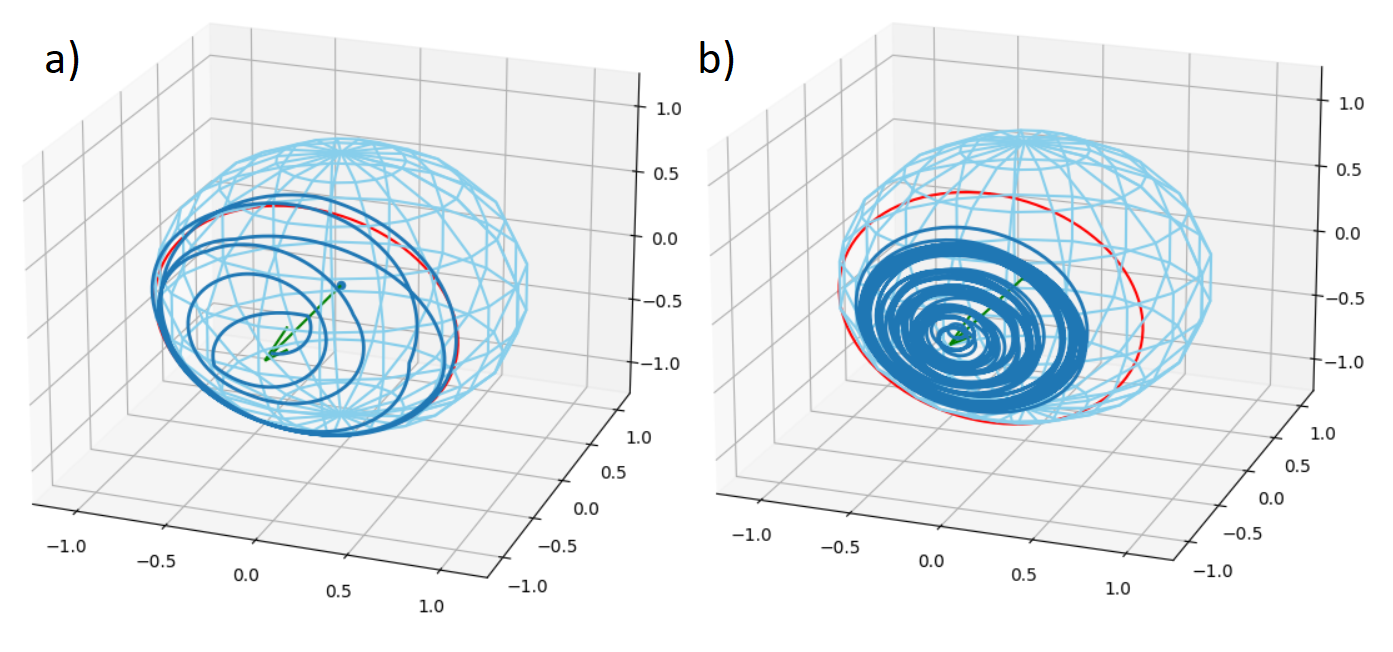
\includegraphics[width = 16cm, height = 7.49cm]{img/Bloch_Sphere_0,4.png}
		\caption{Сфера Блоха, ${\omega}{\tau} = 0.4$ . Красная окружность - зона, при выходе из которой спин отрелаксировал. Внешнее поле больше случайного в a) 5 раз b) в 20 раз. }
		\label{fig:f5}
	\end{figure}
	С помощью программы снимем зависимость времени релаксации от отношения величины внешнего поля к случайному, опять используя размерность $\frac{1}{\omega}$ по оси времени (рис. \ref{fig:f6}). При малом внешнем поле, как видно из графика без внешнего поля, чем больше ${\omega}{\tau}$, тем меньше время релаксации, но скорость его увелечения больше при увелечении внешнего поля.
	\begin{figure}[h!]
		\centering
		\includegraphics[width = 16cm, height = 8.57cm]{img/external_field_plot.png}
		\caption{Зависимость времени релаксации от отношения величины внешнего магнитного поля к случайному}
		\label{fig:f6}
	\end{figure}
	В теории эта зависимость описывается формулой: ${\tau_s}^2 = {{\tau_{s0}}^2}\cdot{(1+({{\Omega}_{outside}\tau})^2)}$ , где $\tau_{s0}$ - время релаксации при отсутствии внешнего поля. Но, построив график ${{\tau_s}^2}/{{\tau_{s0}}^2}$ от $({{\Omega}_{outside}\tau})^2$ (рис. \ref{fig:f7}) , видно, что он не линеен (а в теории ${{\tau_s}^2}/{{\tau_{s0}}^2} = {(1+({{\Omega}_{outside}\tau})^2)}$).
	\begin{figure}[h!]
		\centering
		\includegraphics[width = 16cm, height = 8.52cm]{img/external_field_factor_plot.png}
		\caption{Зависимость ${{\tau_s}^2}/{{\tau_{s0}}^2}$ от $({{\Omega}_{outside}\tau})^2$ растёт быстрее прямой}
		\label{fig:f7}
	\end{figure}
	Можно построить график $ln(\tau_s)$ от $({{\Omega}_{outside}\tau})^2$ (рис. \ref{fig:f8}) . Этот график линеен, откуда можно сделать вывод, что $\tau_s ~ e^{({{\Omega}_{outside}\tau})^2}$ .
	\begin{figure}[h!]
		\centering
		\includegraphics[width = 16cm, height = 8.65cm]{img/external_field_log_plot.png}
		\caption{График $ln(\tau_s)$ от $({{\Omega}_{outside}\tau})^2$ линеен}
		\label{fig:f8}
	\end{figure}
\end{document} 